\thispagestyle{empty}
 \begin{center}
{\bf \TITLE}\\
{
%Tim Menzies, IEEE Fellow, NC State
}
 \end{center}
\vspace{-3mm}
\noindent
%(In this section, all terms shown in {\bf {\em bold font}} are explained later in this proposal.)

Machine learning models, such as deep neural networks (DNNs), are widely used in many industries and businesses such as supply chain, image  recognition, medical diagnosis and autonomous driving. Significant progress has been made by improving the accuracy of DNN models to boost their productivity. 
However, prior work has shown that high accuracy of a model does not imply high robustness (i.e., consistent performance while being tested on new and future datasets). This is because the input data and the external environment (e.g., software and hardware configurations) for a deployed model are constantly changing. 
Hence, ensuring robustness and trustworthiness of deep learning is not an option but a priority to enhance business and consumer confidence.
The results from our previous work have shown that class imbalance~\cite{shumsr22}, data drifting~\cite{majumder2022methods} and software configurations~\cite{xiao2021nondeterministic} can have significant impacts on the robustness and resilience of a model. Our pilot study in Table~\ref{fig:motivation} also conforms that a variety of factors can yield big performance variances when training AI models, which can  impact many CSIRO's missions~\cite{csiromission}.

Our previous efforts in efficiently finding best models (e.g., Dazzle~\cite{shumsr22} to tackle data imbalance and FLASH~\cite{nair2018finding} to tackle highly configurable systems), have paved the way for the understanding of model robustness, however, they are still insufficient in the presence of dynamically changing data and external environments.
Any trusted and accurate model $f$ trained in the past may not be resilient to accurately predict the unseen future data. 
Given a DNN model $\mathbb{Y} = f_\theta(\mathbb{X})$ which is trained to capture relations between the existing data $\mathbb{X}$ and their labels $\mathbb{Y}$ under a particular model configuration $\theta$, the model $f$ together with its configuration (e.g., hyperparameters) needs to be constantly updated to determine the best possible decision boundary by recognizing new data to maintain its best performance.
Unfortunately, retraining the entire model using new and existing data is very costly, while configuration updates are much cheaper to adjust the model performance.

The previous approaches have been exclusively focusing on either data or model configurations to discover issues in learning models, and the structure of DNNs are often ignored (treated as a blackbox) when pinpointing issues or mitigating variances.
In this proposal, we aim to investigate a holistic approach by providing mitigation choices of robustness issues for end-users. For example, stressing more updating configuration $\theta$ than updating data $\mathbb{X}$ by exploring internal structure of DNN using static symbolic techniques to find the sweet spot for updating model in the presence of dynamically  changing data. 

This proposal will allow AI practitioners and domain experts/researchers to build a predictive and responsible foundation by testing, mitigating, and certifying deep learning models in the presence of dynamically changing data. 
%Our previous approach which treats the model as a black box for searching and mitigating model performance fails to examine the internal structure of DNN models, hence can not provide precise predictive robustness and fine-grained robustness guarantee.
Our approach called \mbox{AIEnvelope} aims to develop (1) a predictive foundation to discover emerging robustness issues by considering both data and model configurations.
(2) mitigation methods to repair robustness issues by supporting less-but-high-quality adversarial data to the best possible configurations.
(3) robustness-preserving model reduction approach to reduce high-cost of robust training and (4) quantitative robustness certification with static symbolic techniques to provide quantitative robustness guarantee.
To explore this type of predictive robust learning and its mitigation techniques, we will need to achieve the following goals. 
%robustness is a negoiatble design construct
%offer choices of variance and 
%These deep learning models in the downstream tasks are so pervasive that we are often unaware of their presence until bugs occur. A single defect or robustness issue can cause fatal errors in safety-critical systems, such as autonomous driving and medical diagnosis.  

%However, many current DNN models are found to have robustness issues, can be unsatisfiable to user expectations, or are susceptible to cybersecurity attacks~\cite{shu2020omni}. Prior work has shown that these AI systems are vulnerable and suffer from reliability issues (e.g., incorrect recognition results), fairness concerns (e.g., bias against underrepresented groups) or lacking user privacy protection (e.g., privacy leakage). 
%This proposal will study the robustness (e.g., accuracy variance) of deep neural network models and their impact on downstream learning tasks. 
%We will investigate mitigation techniques for vulnerable DNNs through generating adversarial data and software configurations using active semi-supervised learning. The repaired DNN model will then be optimized via robustness-preserving optimization to reduce training cost and certified via symbolic verification techniques to provide a quantitative robustness guarantee.

\begin{formal}\noindent
{\bf Goal 1:} Predictive robust deep learning with future data and configurations.\label{goal1}
\end{formal}
\noindent
Robustness is the most noteworthy, well-defined correctness property for reliable and responsible DNNs, i.e., minor modifications to the (future) inputs of DNNs must not alter its outputs. Assuring robustness is critically important to prevent AI systems from environmental perturbations and adversarial attacks.
DNNs are imperfect and existing learning models often yield imprecise or incorrect outputs for real-world applications~\cite{pham2020problems,xiao2021nondeterministic}. 
For example, multiple identical training procedures can generate different models with different accuracy variances in the presence of various factors including imperfect data~\cite{zhang2019familial,menzies2012promise,shu2020omni} (e.g., limited, weakly-labelled and concept-drifting training samples) and variance caused by software implementation and configurations  (e.g., nondeterministic DL layers, and random weight initialization and floating-point imprecision). 
We aim to understand and assess a range of factors that affect the robustness of DNNs and provide guidelines for later mitigation and repair: 

\begin{formal}\noindent
{\bf Goal 2:} Harnessing imperfect data and configuration to improve robustness.
\end{formal}
\noindent
The objective is to investigate robust adversarial training with data and software configuration augmentation techniques through semi-supervised contrastive-active learning. 
Obtaining high-quality training data is the first step to build a robust deep learning model. Based on different robustness impacting factors studied in \textbf{Goal 1}, we will harvest the imperfect training data using a new contrastive-active learning approach to iteratively select unlabelled program samples with distinctive features. This enables automatic or fast semi-automatic labelling, hence significantly reducing
manual labelling costs and improving data quality and quantity. This goal enhances the accuracy and robustness of the underlying model, however, the overhead incurred to the iterative adversarial training can be high if the network structure is large. Improving training efficiency for large-scale real-world data is crucial to obtain a more robust model under the same training time constraint. This leads to our next goal to improve training efficiency:


\begin{table}[t]
    \centering
    \caption{Deep learning use cases w.r.t data and configurations related to many of the CSIRO's missions.}
\footnotesize
%fix the table
 \begin{threeparttable}
    \begin{tabular}{llll}
        \toprule
        \textbf{Key technologies} &\textbf{Mission related use cases} &  \textbf{Data} & \textbf{Network Architecture}   \\
        \midrule
        (a) & Recycling waste classification & RecycleNet~\cite{trashnet} & ResNet+Attention~\cite{RecycleNet_trash_images} \\ 
        (b) Geospatial data analytics & Food supply chain supporting  & Traffic prediction dataset~\cite{KaggleTraffic} & GRU~\cite{chung2014empirical} \\
        (c) & AI for health surveillance & Physionet 2017 dataset~\cite{clifford2017af} & ResNet~\cite{hannun2019cardiologist} \\
        (d) & AI for flexible electricity systems & Deep-forecast~\cite{ghaderi2017deepforecast} & DL-STF\tnote{1}~\cite{ghaderi2017deepforecast} \\
        (e) & Water quality forecasting & Water Quality Data~\cite{zhang2019ssim} & DualHeadSSIM~\cite{zhang2021dual} \\
        \bottomrule
        
    \end{tabular}
    \begin{tablenotes}
    \item[1] DL-based Spatio-Temporal Forecasting (DL-STF) denotes the spatio-temporal recurrent neural network in~\cite{ghaderi2017deepforecast}.
  \end{tablenotes}
    \end{threeparttable}
\label{tab:existing}
\end{table} 

\begin{figure}[t]
    \centering
    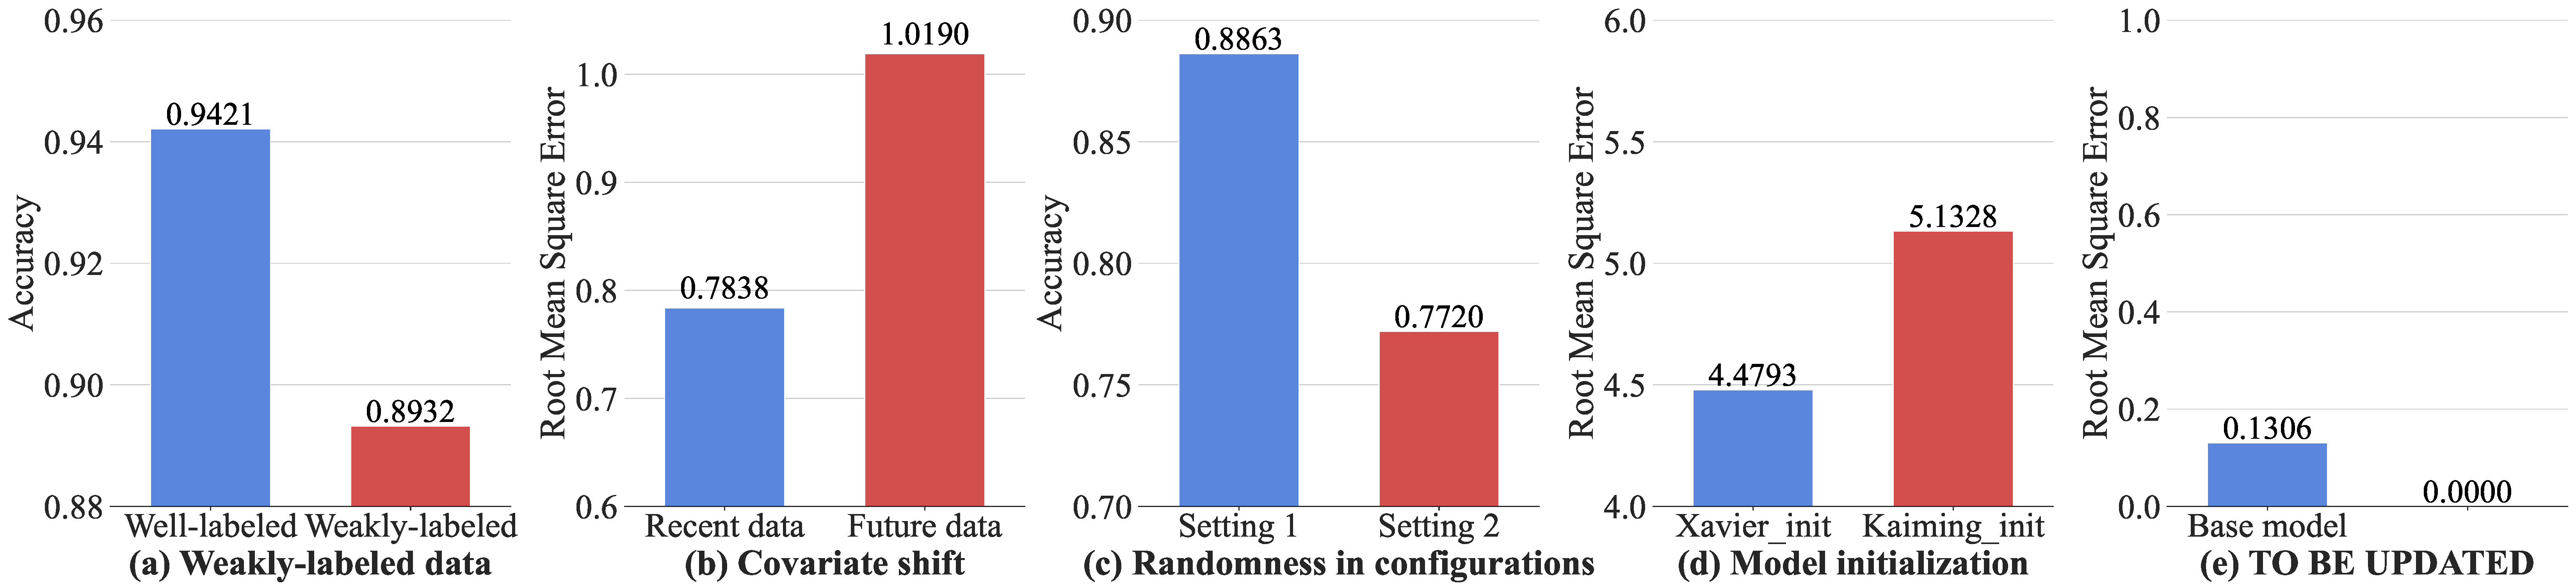
\includegraphics[width=\linewidth]{fig/factors.pdf}
    \caption{Various factors affecting the robustness of deep learning impacting on many of the CSIRO's missions  }
    \label{fig:motivation}
\end{figure}

\noindent
\begin{formal}
{\bf Goal 3:} Model reduction and optimization to  improve training efficiency.
\end{formal}
\noindent
Deep learning models often suffer from redundancy in their network structure, which affects their training efficiency. For example, the over-fitting issue in DNNs~\cite{denil2013predicting} has shown that a large proportion of the configuration parameters are not contributed to the model robustness. 
In this goal, we aim to perform model reduction and optimization to improve training efficiency. Specifically, our novelty lies in robustness-preserved structure transformation to perform network pruning~\cite{han2015learning,luo2017thinet} and  quantize~\cite{ullrich2017soft} through hyperparameter tuning, quantization, parallelism.
The model is reduced and optimized where necessary but preserving the same robustness to boost the adversarial training in \textbf{Goal 2}. Though model reduction (\textbf{Goal 3}) and robustness repair (\textbf{Goal 2}) complement each other, they can be conducted iteratively with one's output as the other's input to continuously improve the overall robustness.
With all that done, we will conduct the final verification to qualitatively certify the underlying DNN model: 
  \noindent
\begin{formal}
{\bf Goal 4:} Quantitative robustness certification of DNN models. 
\end{formal}
\noindent  
Given a repaired and reduced DNN model from \textbf{Goal 2} and \textbf{Goal 3}, our final aim is to conduct precise verification of DNNs using symbolic quantitative certification for the robustness property of the model. 
In the verification of neural networks, a simple yes/no to a verification result about the robustness cannot demonstrate the confidence of the model (e.g., how many perturbed inputs change the model and how much of the deviation of the model has changed). To quantitatively measure and compare the performances of the models by giving in numerous domains would extend the measurement, compared with a threshold deemed with a certain region in a confidence interval. 

